% !TEX encoding = UTF-8
% !TEX TS-program = pdflatex
% !TEX root = ../tesi.tex
\newpage
\section{Codifica}\label{sec:codifica}
Per la fase di codifica sono state adottate le seguenti convenzioni:
\begin{itemize}
    \item il nome delle classi seguirà la notazione a Cammello, un esempio corretto è: \textit{WindowsCommandFactory};
    \item il nome degli attributi seguirà sempre la notazione a Cammello, ma con la prima lettera in minuscolo, un esempio corretto è: \textit{commandsFactory};
    \item ove possibile, si deve utilizzare le espressioni lambda;
    \item la gestione delle eccezioni deve essere venir fatta sempre dal chiamante;
    \item per ogni classe e ogni metodo deve essere fornita una descrizione in JavaDoc.
\end{itemize}
\subsection{Inizializzazione View}\label{subsec:inizializzazione-view}
Il seguente segmento del codice è necessario per creare completare la relazione di osservazione che esiste tra la View e il Model.
\begin{lstlisting}[caption={Inizializzazione relazione di osservazione View e Model},label={lst:lstlisting}]
model.getApkName().observe(newValue -> {
    view.getPackageInfo().setText(newValue);
    view.getBtnStartDecompile().setEnabled(!newValue.equalsIgnoreCase(""));
});
model.getAvdList().observe(lis -> view.getCbAvdList().setModel(new DefaultComboBoxModel<>(lis)));
model.getIsDecompiled().observe(newValue -> {
    JButton[] controlledButtons = view.getControlledButtons();
    for (JButton controlledButton : controlledButtons) controlledButton.setEnabled(newValue);
});
\end{lstlisting}
Nella View è presente un'eticchetta che mostra il file APK selezionato da decompilare, questa componente della view osserva l'attributo \textit{apkName} del modello, e una volta selezionato il file, viene ottenuto il path del file APK e aggiornato il modello, l'etichetta riceverà la notifica con il path aggiornato.

\subsection{Analisi del codice e generazione del pdf}\label{subsec:analisi-del-codice-e-generazione-del-pdf}
Dopo aver decompilato un file \textit{.apk}, e decodificato i file \textit{dex} l'utente può scegliere di effettuare l'operazione di analisi offerta dal tool.
Questa funzionalità si deve istanziare un oggetto di tipo BaseAnalyzer, e in base alle opzioni di analisi che l'utente ha scelta dalla vista:
\begin{figure}[H]
    \centering
    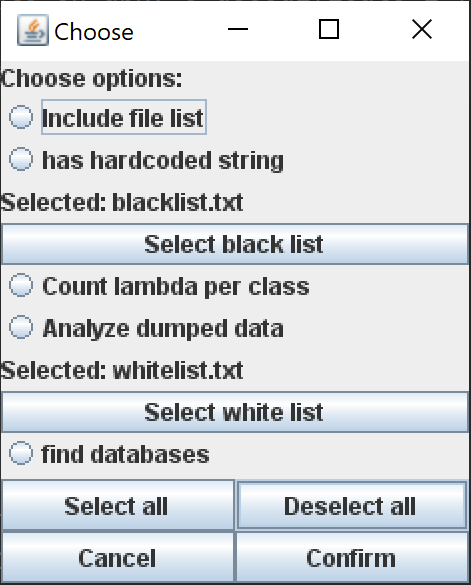
\includegraphics{./immagini/tool/analysis_chooser.png}
    \caption{Schermata delle opzioni dell'analisi}\label{fig:analysis_chooser}
\end{figure}
Di seguito è il codice che si occupa di "decorare" l'oggetto base, effettuare l'analisi e quindi generare un file pdf contenente il risultato:

\begin{lstlisting}[caption={Decorator},label={lst:analyze}]
public void analyze(Map< String, Boolean > thingsTodo, File blackList, File whiteList) {
...
Analyze analyze = new BaseAnalyzer(thingsTodo.get(AnalysisChooser.LIST_FILE), decompiledFiles);
...
// se analyzeString==true, allora analizzo le stringhe
if (thingsTodo.get(AnalysisChooser.FIND_STRING))
    analyze = new StringFinder(analyze, blackList);
if (thingsTodo.get(AnalysisChooser.COUNT_LAMBDA))
    analyze = new LambdaCounter(analyze);
if (thingsTodo.get(AnalysisChooser.DUMPED_FILE))
    analyze = new DumpedFilesAnalyzer(analyze, whiteList);
if (thingsTodo.get(AnalysisChooser.LIST_DBS))
    analyze = new DumpDataBase(analyze);
...
PDFWriter pdfWriter = new PDFWriter(resultFile);
pdfWriter.addParagraphs(analyze.getResult());
...
}
\end{lstlisting}

Con l'utilizzo del pattern decorator \`{e} estremamente semplice aggiungere un tipo di analisi, poiché è sufficiente aggiungere nella map \textit{thingsToDo} al momento della chiamata del metodo \textit{analyze}, creare una nuova classe che eredita dalla classe base dei decorator implementandone il metodo astratto e aggiungere due righe d'istruzione.

\subsection{Istanziazione di Commands}\label{subsec:istanziazione-di-commands}
Per il corretto funzionamento del tool è necessario che all'avvio venga instanziata una delle seguenti classi:
\begin{itemize}
    \item WindowsCommandFactory;
    \item LinuxCommandFactory.
\end{itemize}
Il seguente segmento di codice risolve tale problema:

\begin{lstlisting}[caption={Creazione dell'istanza di Commands in base al S.O.},label={lst:commands}]
Commands commands;
String osInfo = System.getProperty("os.name");
if (containsIgnoreCase(osInfo, "windows")) {
    commands = new WindowsCommandFactory(model.getBasePath().getValue(), "cmd.exe", "/c");
} else {
    commands = new UnixCommandFactory(model.getBasePath().getValue(), "bash", "-c");
}
Controller controller = new Controller(model, commands);
\end{lstlisting}